\documentclass[11pt]{article}

\usepackage[margin=1in]{geometry}
\usepackage[T1]{fontenc}
\usepackage[utf8]{inputenc}
\usepackage{graphicx}
\usepackage{booktabs}
\usepackage{amsmath}
\usepackage{hyperref}
\usepackage{url}

\graphicspath{{figures/}}

\title{Stiffness-Modulated Harmonic Priors for Molecular Conformation Flow Matching: A Full-Database Evaluation}
\author{Final Project Report}
\date{May 2026}

\begin{document}

\maketitle

\begin{abstract}
Molecular conformer generation requires models that can produce geometrically plausible structures while preserving enough diversity to cover reference conformer ensembles. This project studies a source-only intervention for Cartesian flow matching under a fixed model architecture and objective. The main idea is to combine a strong harmonic prior, which gives a global source distribution, with local stiffness rules that reduce perturbations around rigid chemistry and allow larger perturbations around flexible regions. On the full-database GEOM-Drugs setting used in this project, local stiffness structure alone improves over isotropic and torsion-only sources on tracked validation and single-sample RMSD metrics, but it does not replace the harmonic prior. The strongest validation/RMSD result comes from a stiffness-modulated harmonic source with $\lambda=5.0$, trained with AdamW at learning rate $10^{-3}$; this setting beats optimized harmonic on tracked loss/RMSD metrics across random and scaffold splits and seeds 0, 1, and 2. Complete val/test COV/AMR evaluation gives a more nuanced conclusion. The high-lambda hybrid strongly improves AMR-P precision, while lower $\lambda$ better preserves recall. The best tested hybrid recall/balanced setting is $\lambda=0.025$, and harmonic remains the AMR-R recall anchor in the harmonic-vs-hybrid comparison. The final conclusion is therefore not universal dominance by one lambda, but a tunable precision-recall frontier induced by stiffness-modulated harmonic priors.
\end{abstract}

\section{Introduction}

Molecular conformer generation is the task of producing plausible three-dimensional arrangements for a fixed molecular graph. This problem matters because many molecular properties depend on accessible conformations rather than on graph topology alone. For drug-like molecules, a useful conformer generator must do more than minimize a single RMSD value: it should produce chemically reasonable structures and should cover the relevant conformational ensemble.

This project focuses on fixed-topology conformer generation with Cartesian flow matching. In this setting, the model learns a velocity field between a source geometry $x_0$ and a target conformer $x_1$, commonly through a linear interpolation
\begin{equation}
    x_t = (1-t)x_0 + t x_1 .
\end{equation}
The source distribution is therefore a central design choice. If the source is too naive, the model may waste capacity learning to repair unphysical bond, angle, or ring distortions. If the source is too restrictive, sampling may become precise but insufficiently diverse. The question is not only whether a source makes training loss lower, but also how it changes the precision and recall of generated conformer ensembles.

Naive isotropic Cartesian corruption is limited because it treats every atom and local chemical environment similarly. That is a poor match to molecular geometry. Bonds, rings, and amide-like motifs are relatively stiff, while rotatable bonds and terminal flexible groups support much larger variation. Torsion-focused methods highlight the importance of soft degrees of freedom \cite{torsionaldiffusion}, but a torsion-only source may not provide enough global geometric structure. Harmonic priors, as used in ET-Flow-style Cartesian conformer generation, are strong because they provide a global low-energy-like source geometry while staying in Cartesian coordinates \cite{etflow}. This project asks whether local stiffness information can improve that harmonic prior rather than replace it.

The main research question is:

\begin{quote}
Can local stiffness rules improve a strong harmonic/global prior under a fixed Cartesian flow-matching setup, and how does this affect precision versus recall in conformer ensemble evaluation?
\end{quote}

The final answer is mixed but useful. Local stiffness structure improves over weaker source baselines on tracked training and single-sample metrics. When stiffness modulation is combined with the harmonic prior, the high-lambda hybrid gives the best validation and single-sample RMSD results. However, complete val/test COV/AMR evaluation shows that this improvement is precision-favorable rather than universally ensemble-optimal. The final contribution is best framed as a tunable source-prior family that exposes a precision-recall tradeoff.

\section{Background and Method}

\subsection{Flow Matching Setup}

The project keeps the backbone, objective, and training design fixed across the main comparisons. For each molecule, the model observes a molecular graph and a reference conformer representation. A source geometry $x_0$ is sampled from a chosen source construction, and the target geometry $x_1$ is a training conformer. The interpolation path is Cartesian and linear:
\begin{equation}
    x_t = (1-t)x_0 + t x_1,
\end{equation}
with a corresponding velocity target determined by the displacement from source to target. The model is then trained to predict this velocity field from the interpolated geometry and molecular information.

This setup deliberately avoids a full internal-coordinate probability path. That choice keeps the attribution clean: differences between methods should come from the source construction rather than from a new backbone or objective. It also avoids fragile coordinate reconstruction chains, which can make molecular validity harder to interpret.

\subsection{Source Corruption Baselines}

The final optimized all-method matrix compares five source constructions.

\paragraph{Isotropic source.}
The isotropic baseline applies generic Cartesian perturbations without encoding local chemistry. It is useful as a naive lower baseline because it tests whether simply adding coordinate noise is enough.

\paragraph{Torsion-only source.}
The torsion-only baseline focuses perturbation on flexible torsional degrees of freedom. It reflects the idea that conformational variation is often concentrated in rotations around soft bonds. In the final results, torsion-only behaves as a recall-biased but precision-poor baseline.

\paragraph{Stiffness-structured source.}
The stiffness-structured source uses heuristic local chemistry classes. Rigid or sensitive regions such as rings, amide-like motifs, aromatic or conjugated regions when detectable, and bond/angle-sensitive neighborhoods receive smaller perturbations. Flexible regions such as rotatable-bond neighborhoods and terminal groups receive larger perturbations. This source tests whether local stiffness alone improves over generic corruption.

\paragraph{Harmonic prior.}
The harmonic prior is the strongest non-hybrid source baseline in the tracked validation/RMSD experiments. It provides a global source geometry and is closer in spirit to ET-Flow-style Cartesian conformer generation \cite{etflow}. Earlier experiments showed that stiffness structure alone was useful but weaker than the harmonic prior, motivating a hybrid rather than a replacement.

\subsection{Stiffness-Modulated Harmonic Prior}

The hybrid source keeps the harmonic prior as the global source distribution and applies local stiffness modulation conservatively. A useful idealized form is
\begin{equation}
    x_0 = x_{\mathrm{ref}} + L_{\mathrm{harm}} D_{\mathrm{stiff}}(\lambda)^{1/2} z,
    \label{eq:hybrid-source}
\end{equation}
where $x_{\mathrm{ref}}$ is a reference geometry, $L_{\mathrm{harm}}$ represents the global harmonic source transform, $z$ is standard noise, and $D_{\mathrm{stiff}}(\lambda)$ is a local modulation term controlled by the stiffness classes. In words, the harmonic prior determines the overall source structure, while the stiffness rule changes the local scale of perturbations.

This design was chosen for attribution. It does not claim to learn force constants or perform full physical normal-mode sampling. It only asks whether a simple local chemical rule can improve a strong harmonic source under the same flow-matching training setup.

\subsection{Lambda as a Modulation Parameter}

The parameter $\lambda$ controls the strength of local stiffness modulation. Small $\lambda$ keeps the source close to the harmonic prior, while larger $\lambda$ makes local stiffness rules more influential. Because stiffness modulation can reduce variation in rigid regions and shift variation toward flexible regions, it can plausibly change both precision and recall. A high value may generate structures that are closer to a preferred local geometry, improving precision-style metrics. The same behavior can reduce coverage of the reference ensemble, hurting recall-style metrics. The final COV/AMR results support exactly this interpretation.

\section{Experimental Setup}

\subsection{Dataset and Splits}

The final experiments use the full-database GEOM-Drugs setting prepared in this repository \cite{geom}. Training and reporting reuse cached processed artifacts and cached random/scaffold splits. The optimized training summaries cover both random and Bemis-Murcko scaffold splits, with seeds 0, 1, and 2. The COV/AMR evaluation uses val/test partitions only, not train, because including the train partition would substantially increase the evaluation cost and was not needed for the final model-selection question.

The complete hybrid-lambda COV/AMR evaluation reports 60,868 planned molecule slots and 1,095,624 evaluated method-seed-molecule records, with no missing chunk files and no failed or skipped records in the final merged summary. Each evaluated molecule uses $K=20$ generated conformers, and COV uses an RMSD threshold $\delta=0.75$.

\subsection{Methods Compared}

The final optimized all-method training matrix compares:
\begin{itemize}
    \item isotropic,
    \item torsion-only,
    \item stiffness-structured,
    \item harmonic-prior,
    \item \texttt{hybrid\_harmonic\_stiffness\_v1} with $\lambda=5.0$.
\end{itemize}

The final hybrid-lambda COV/AMR comparison includes harmonic as the $\lambda=0$ reference and hybrid lambdas 0.025, 0.1, 1.0, 3.0, and 5.0. Old SGD-trained lambda runs and superseded summaries are not used as final evidence.

\subsection{Training Protocol}

The final optimized training protocol uses AdamW with learning rate $10^{-3}$. This setting was selected by an optimizer/LR pilot that compared SGD and AdamW variants. The model architecture, checkpoint/reload behavior, validation-driven checkpoint selection, one-step sampling diagnostics, and hard step cap are held fixed across the final method matrix. The final optimized all-method summary reports 30/30 expected result JSONs available.

\subsection{Metrics}

The tracked training and sampling metrics are best validation loss, reloaded validation loss, and sampled RMSD to target overall and by train/val/test partition. These metrics are useful for optimization and single-sample quality, but they do not fully characterize conformer-ensemble behavior.

The ensemble evaluation uses COV/AMR:
\begin{itemize}
    \item COV-R and AMR-R are recall-style metrics. They measure how well generated conformers cover the reference ensemble.
    \item COV-P and AMR-P are precision-style metrics. They measure how close generated conformers are to reference structures.
\end{itemize}
Higher COV is better, while lower AMR is better. The final interpretation depends on considering both types of metrics together.

The final reports remain non-benchmark. PoseBusters-style, MMFF/UFF, and xTB physical benchmark validation was planned but not completed as final evidence. This limitation matters because RMSD and COV/AMR do not replace physical validity checks \cite{posebusters}.

\section{Results}

\subsection{Stiffness Alone Improves Over Isotropic and Torsion-Only}

The stiffness-structured source improves over isotropic and torsion-only sources on the final optimized tracked validation/RMSD metrics. Across random and scaffold splits, the stiffness-structured source has a lower cross-split mean best validation loss than isotropic, and a much lower sampled RMSD than torsion-only. This supports the basic premise that local stiffness structure is useful.

However, stiffness structure alone is not the strongest source. The harmonic prior has a lower cross-split mean best validation loss and lower sampled RMSD than stiffness-structured corruption. This was the key reason to move from a ``stiffness replaces harmonic'' question to a ``stiffness improves harmonic'' question.

\begin{table}[t]
\centering
\small
\caption{Final optimized tracked-metric ordering under AdamW with learning rate $10^{-3}$. Values are cross-split means over random and scaffold splits and seeds 0, 1, and 2. Lower is better for validation loss and RMSD.}
\label{tab:optimized-ordering}
\begin{tabular}{lrrrr}
\toprule
Method & Best val. loss & Reloaded val. loss & RMSD overall & RMSD test \\
\midrule
Hybrid $\lambda=5.0$ & 0.01198 & 0.01198 & 0.08991 & 0.09161 \\
Harmonic prior & 0.01840 & 0.01840 & 0.11630 & 0.11661 \\
Stiffness structured & 0.04710 & 0.04710 & 0.18266 & 0.18423 \\
Isotropic & 0.06221 & 0.06221 & 0.21592 & 0.21590 \\
Torsion only & 4.01619 & 4.01619 & 1.80419 & 1.73375 \\
\bottomrule
\end{tabular}
\end{table}


\subsection{Hybrid Lambda 5 Improves Optimized Tracked Loss/RMSD}

Under the final AdamW lr $10^{-3}$ protocol, the high-modulation hybrid with $\lambda=5.0$ is the strongest method on tracked validation/RMSD metrics. Its cross-split mean best validation loss is 0.01198, compared with 0.01840 for harmonic. Its cross-split sampled RMSD overall is 0.08991, compared with 0.11630 for harmonic. The final optimized harmonic-vs-hybrid summary reports complete coverage over random and scaffold splits and seeds 0, 1, and 2.

This result is important because it shows that the hybrid gain is not only a scaffold seed0 artifact or an optimizer artifact. After the optimizer pilot selected AdamW lr $10^{-3}$ for both harmonic and hybrid, the hybrid remained better on the tracked core metrics.

\subsection{Full-Method Optimized Ordering}

The final optimized tracked-metric ordering is:
\begin{equation}
\text{hybrid } \lambda=5.0 > \text{harmonic} > \text{stiffness} > \text{isotropic} > \text{torsion-only}.
\end{equation}
This ordering holds qualitatively across the random and scaffold summaries for validation loss and single-sample RMSD. Figure~\ref{fig:method-comparison} gives the final method-level comparison used in the reporting bundle.

\begin{figure}[t]
    \centering
    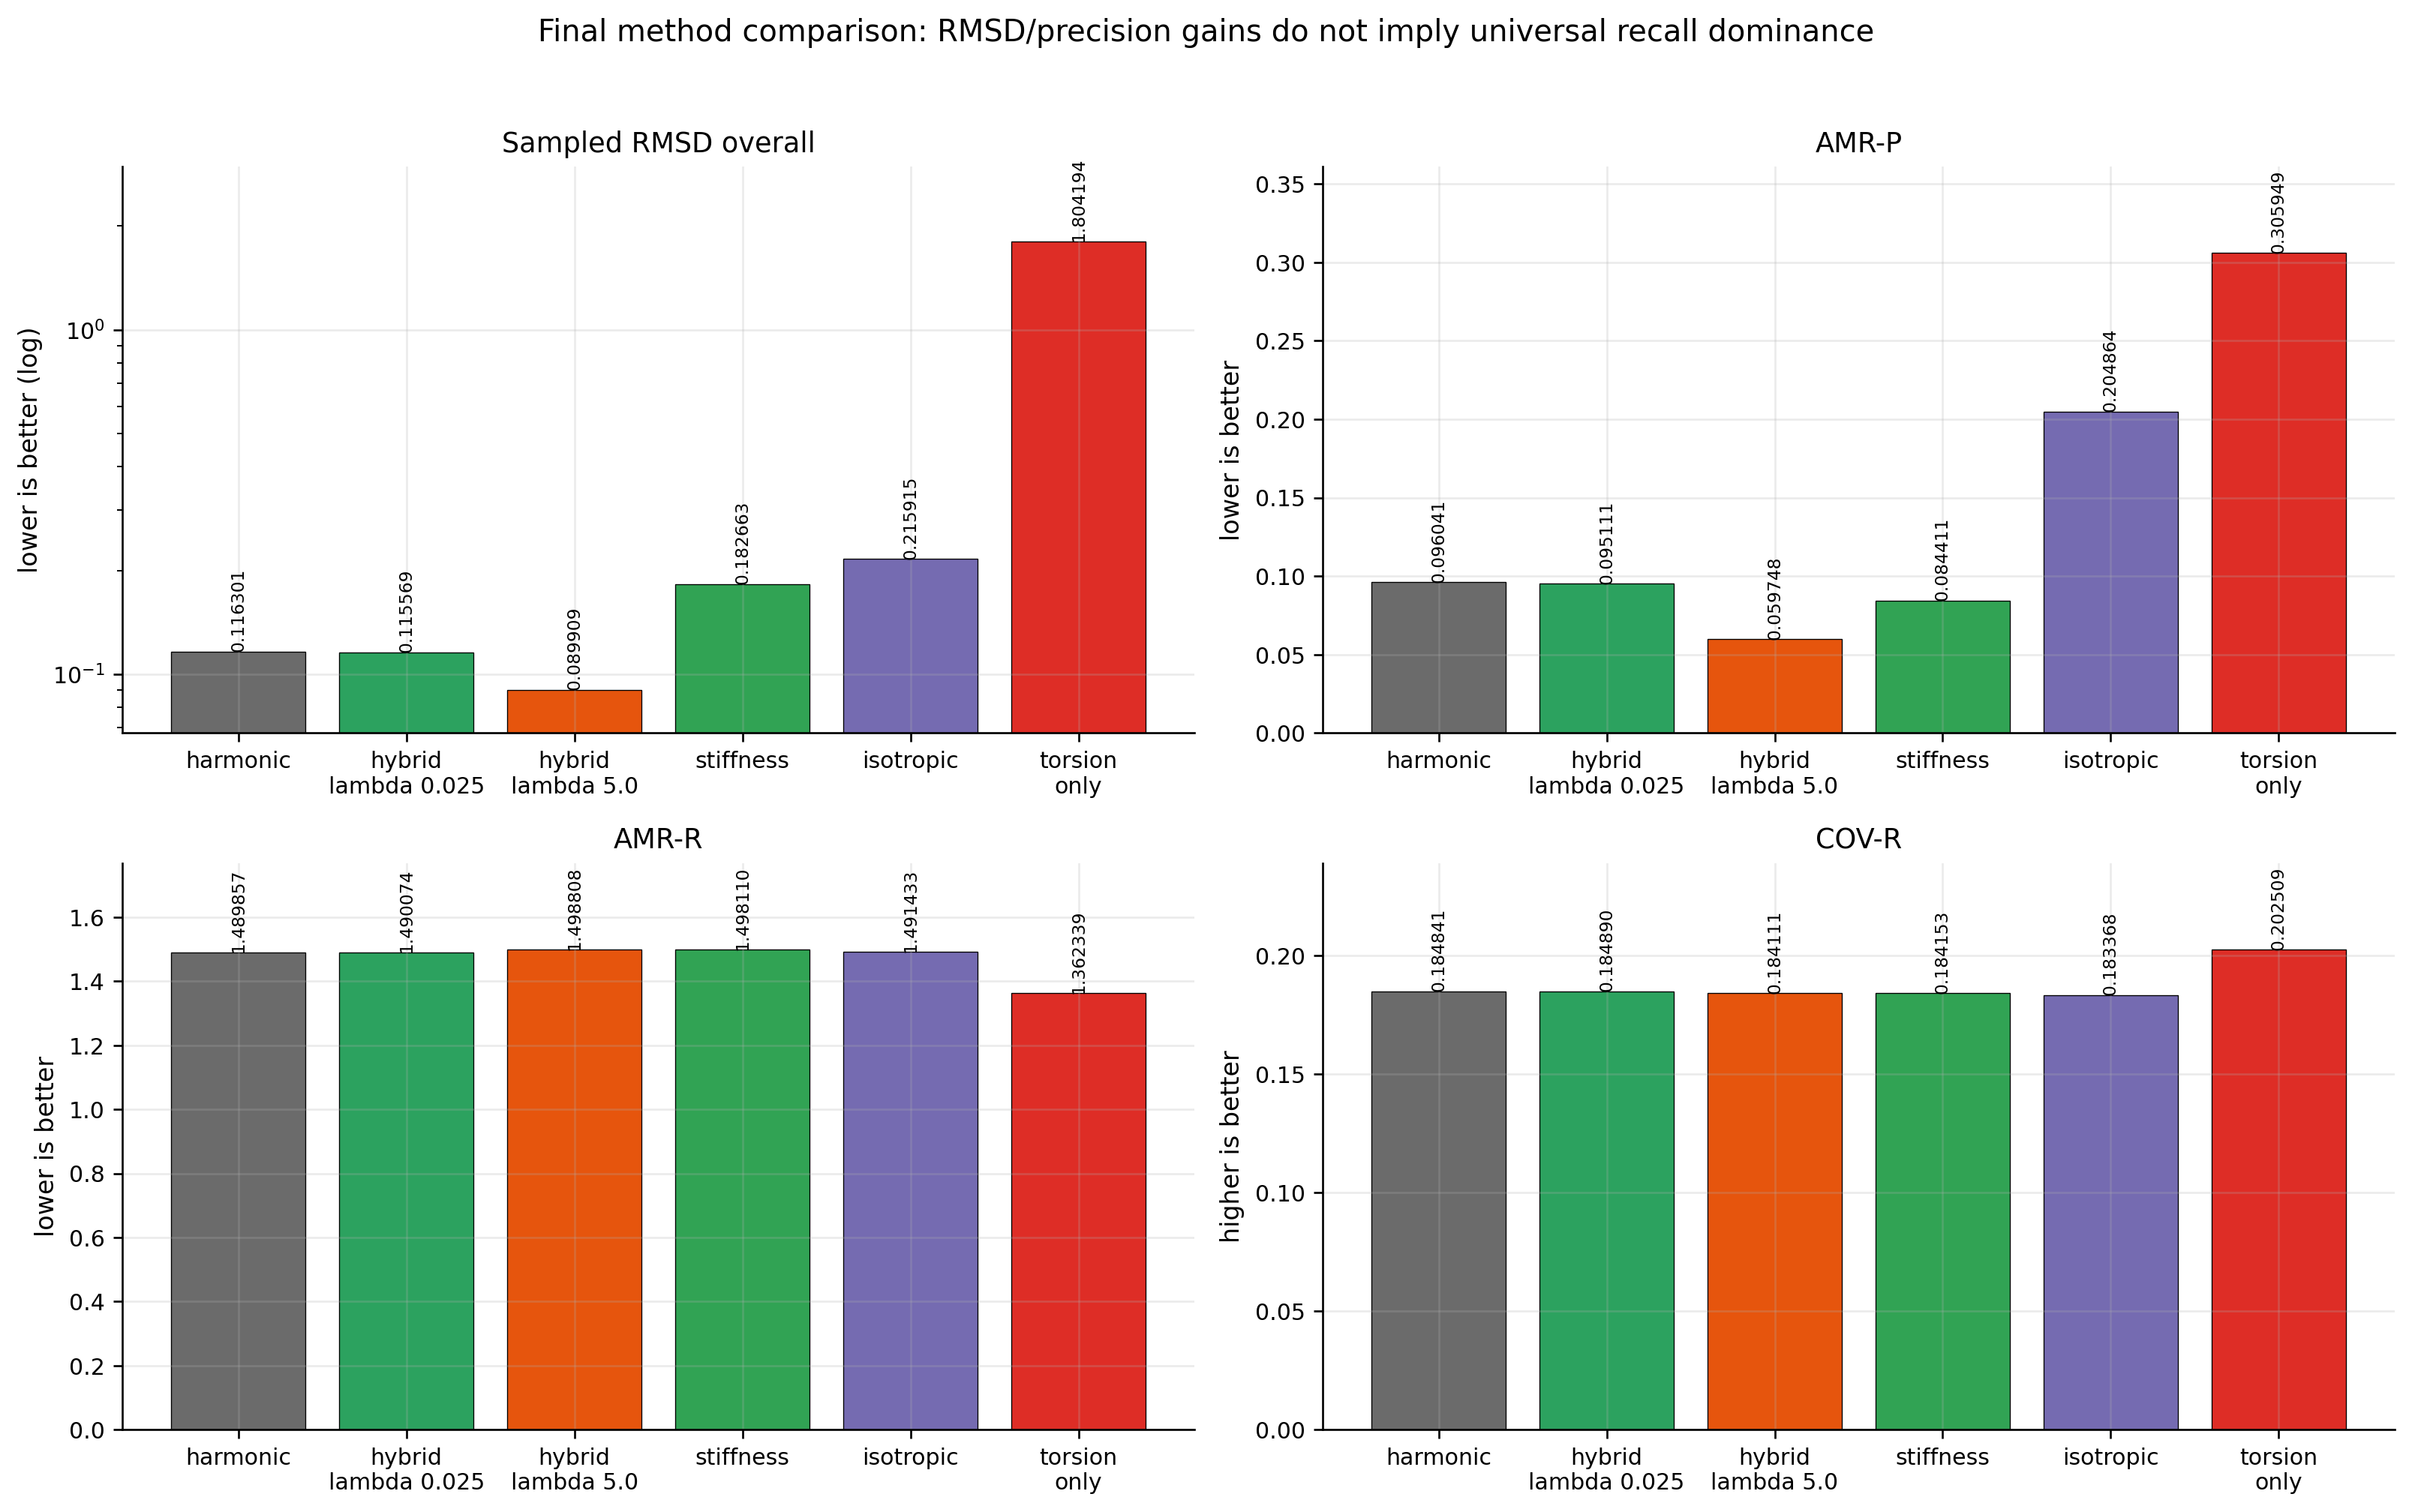
\includegraphics[width=0.95\linewidth]{geom_full_database_final_method_comparison_rmsd_cov_amr.png}
    \caption{Final method comparison figure from the closure bundle. The tracked validation/RMSD metrics favor the high-lambda hybrid, while COV/AMR shows a more nuanced precision-recall pattern.}
    \label{fig:method-comparison}
\end{figure}

\subsection{Complete Val/Test COV/AMR Reveals a Precision-Recall Tradeoff}

The complete val/test COV/AMR evaluation changes the interpretation. The high-lambda hybrid remains very strong on AMR-P: $\lambda=5.0$ has AMR-P mean 0.05975, compared with 0.09604 for harmonic. COV-P is saturated at 1.0 for harmonic, stiffness, isotropic, and the high-lambda hybrid, so AMR-P is the more informative precision metric here.

Recall-style metrics tell a different story. In the harmonic-vs-hybrid comparison, harmonic has the best AMR-R mean at 1.48986, while hybrid $\lambda=5.0$ has AMR-R mean 1.49881. COV-R also decreases from 0.18484 for harmonic to 0.18411 for $\lambda=5.0$. These differences are small in absolute scale but systematic in the final summary and point in the same direction: higher stiffness modulation improves precision but weakens recall.

The all-method COV/AMR table also shows why the result should not be compressed into a single scalar winner. Torsion-only has recall-favorable COV-R and AMR-R values but very poor AMR-P and lower COV-P, meaning it covers more reference conformers at the cost of generating less precise structures. This reinforces the need to report precision and recall together.

\begin{table}[t]
\centering
\small
\caption{Complete val/test COV/AMR summary for the final all-method matrix. COV-R and AMR-R are recall-style metrics, while COV-P and AMR-P are precision-style metrics. Higher is better for COV; lower is better for AMR.}
\label{tab:cov-amr-summary}
\begin{tabular}{lrrrr}
\toprule
Method & COV-R & COV-P & AMR-R & AMR-P \\
\midrule
Hybrid $\lambda=5.0$ & 0.18411 & 1.00000 & 1.49881 & 0.05975 \\
Harmonic prior & 0.18484 & 1.00000 & 1.48986 & 0.09604 \\
Stiffness structured & 0.18415 & 1.00000 & 1.49811 & 0.08441 \\
Isotropic & 0.18337 & 1.00000 & 1.49143 & 0.20486 \\
Torsion only & 0.20251 & 0.95970 & 1.36234 & 0.30595 \\
\bottomrule
\end{tabular}
\end{table}


\subsection{Lambda Controls the Pareto Frontier}

The full hybrid-lambda COV/AMR evaluation directly tests whether $\lambda=5.0$ is ensemble-optimal. It is not. Among tested hybrid lambdas, $\lambda=5.0$ is precision-optimal by AMR-P, but $\lambda=0.025$ is recall-optimal among hybrids by COV-R and AMR-R and is also selected as the balanced lambda by rank aggregation over AMR-P, AMR-R, $1-\mathrm{COV\mbox{-}R}$, and $1-\mathrm{COV\mbox{-}P}$.

The trend is monotonic in the main qualitative sense: as $\lambda$ increases, AMR-P improves, while COV-R and AMR-R degrade. All tested hybrid lambdas are reported on the Pareto frontier in the final lambda summary. No tested hybrid lambda improves both precision and recall over harmonic. This is the central result of the project.

\begin{table}[t]
\centering
\small
\caption{Hybrid-lambda COV/AMR interpretation. The harmonic prior is shown as the $\lambda=0$ reference. Higher is better for COV; lower is better for AMR.}
\label{tab:lambda-interpretation}
\begin{tabular}{lrrrrl}
\toprule
Entry & COV-R & COV-P & AMR-R & AMR-P & Interpretation \\
\midrule
Harmonic prior ($\lambda=0$) & 0.18484 & 1.00000 & 1.48986 & 0.09604 & Recall anchor \\
Hybrid $\lambda=0.025$ & 0.18489 & 1.00000 & 1.49007 & 0.09511 & Best hybrid recall/balanced \\
Hybrid $\lambda=0.1$ & 0.18481 & 1.00000 & 1.49059 & 0.09263 & Low-lambda frontier point \\
Hybrid $\lambda=1.0$ & 0.18441 & 1.00000 & 1.49708 & 0.06537 & Mid-lambda frontier point \\
Hybrid $\lambda=3.0$ & 0.18413 & 1.00000 & 1.49855 & 0.06052 & Precision-favorable \\
Hybrid $\lambda=5.0$ & 0.18411 & 1.00000 & 1.49881 & 0.05975 & Precision/RMSD-favorable \\
\bottomrule
\end{tabular}
\end{table}


\begin{figure}[t]
    \centering
    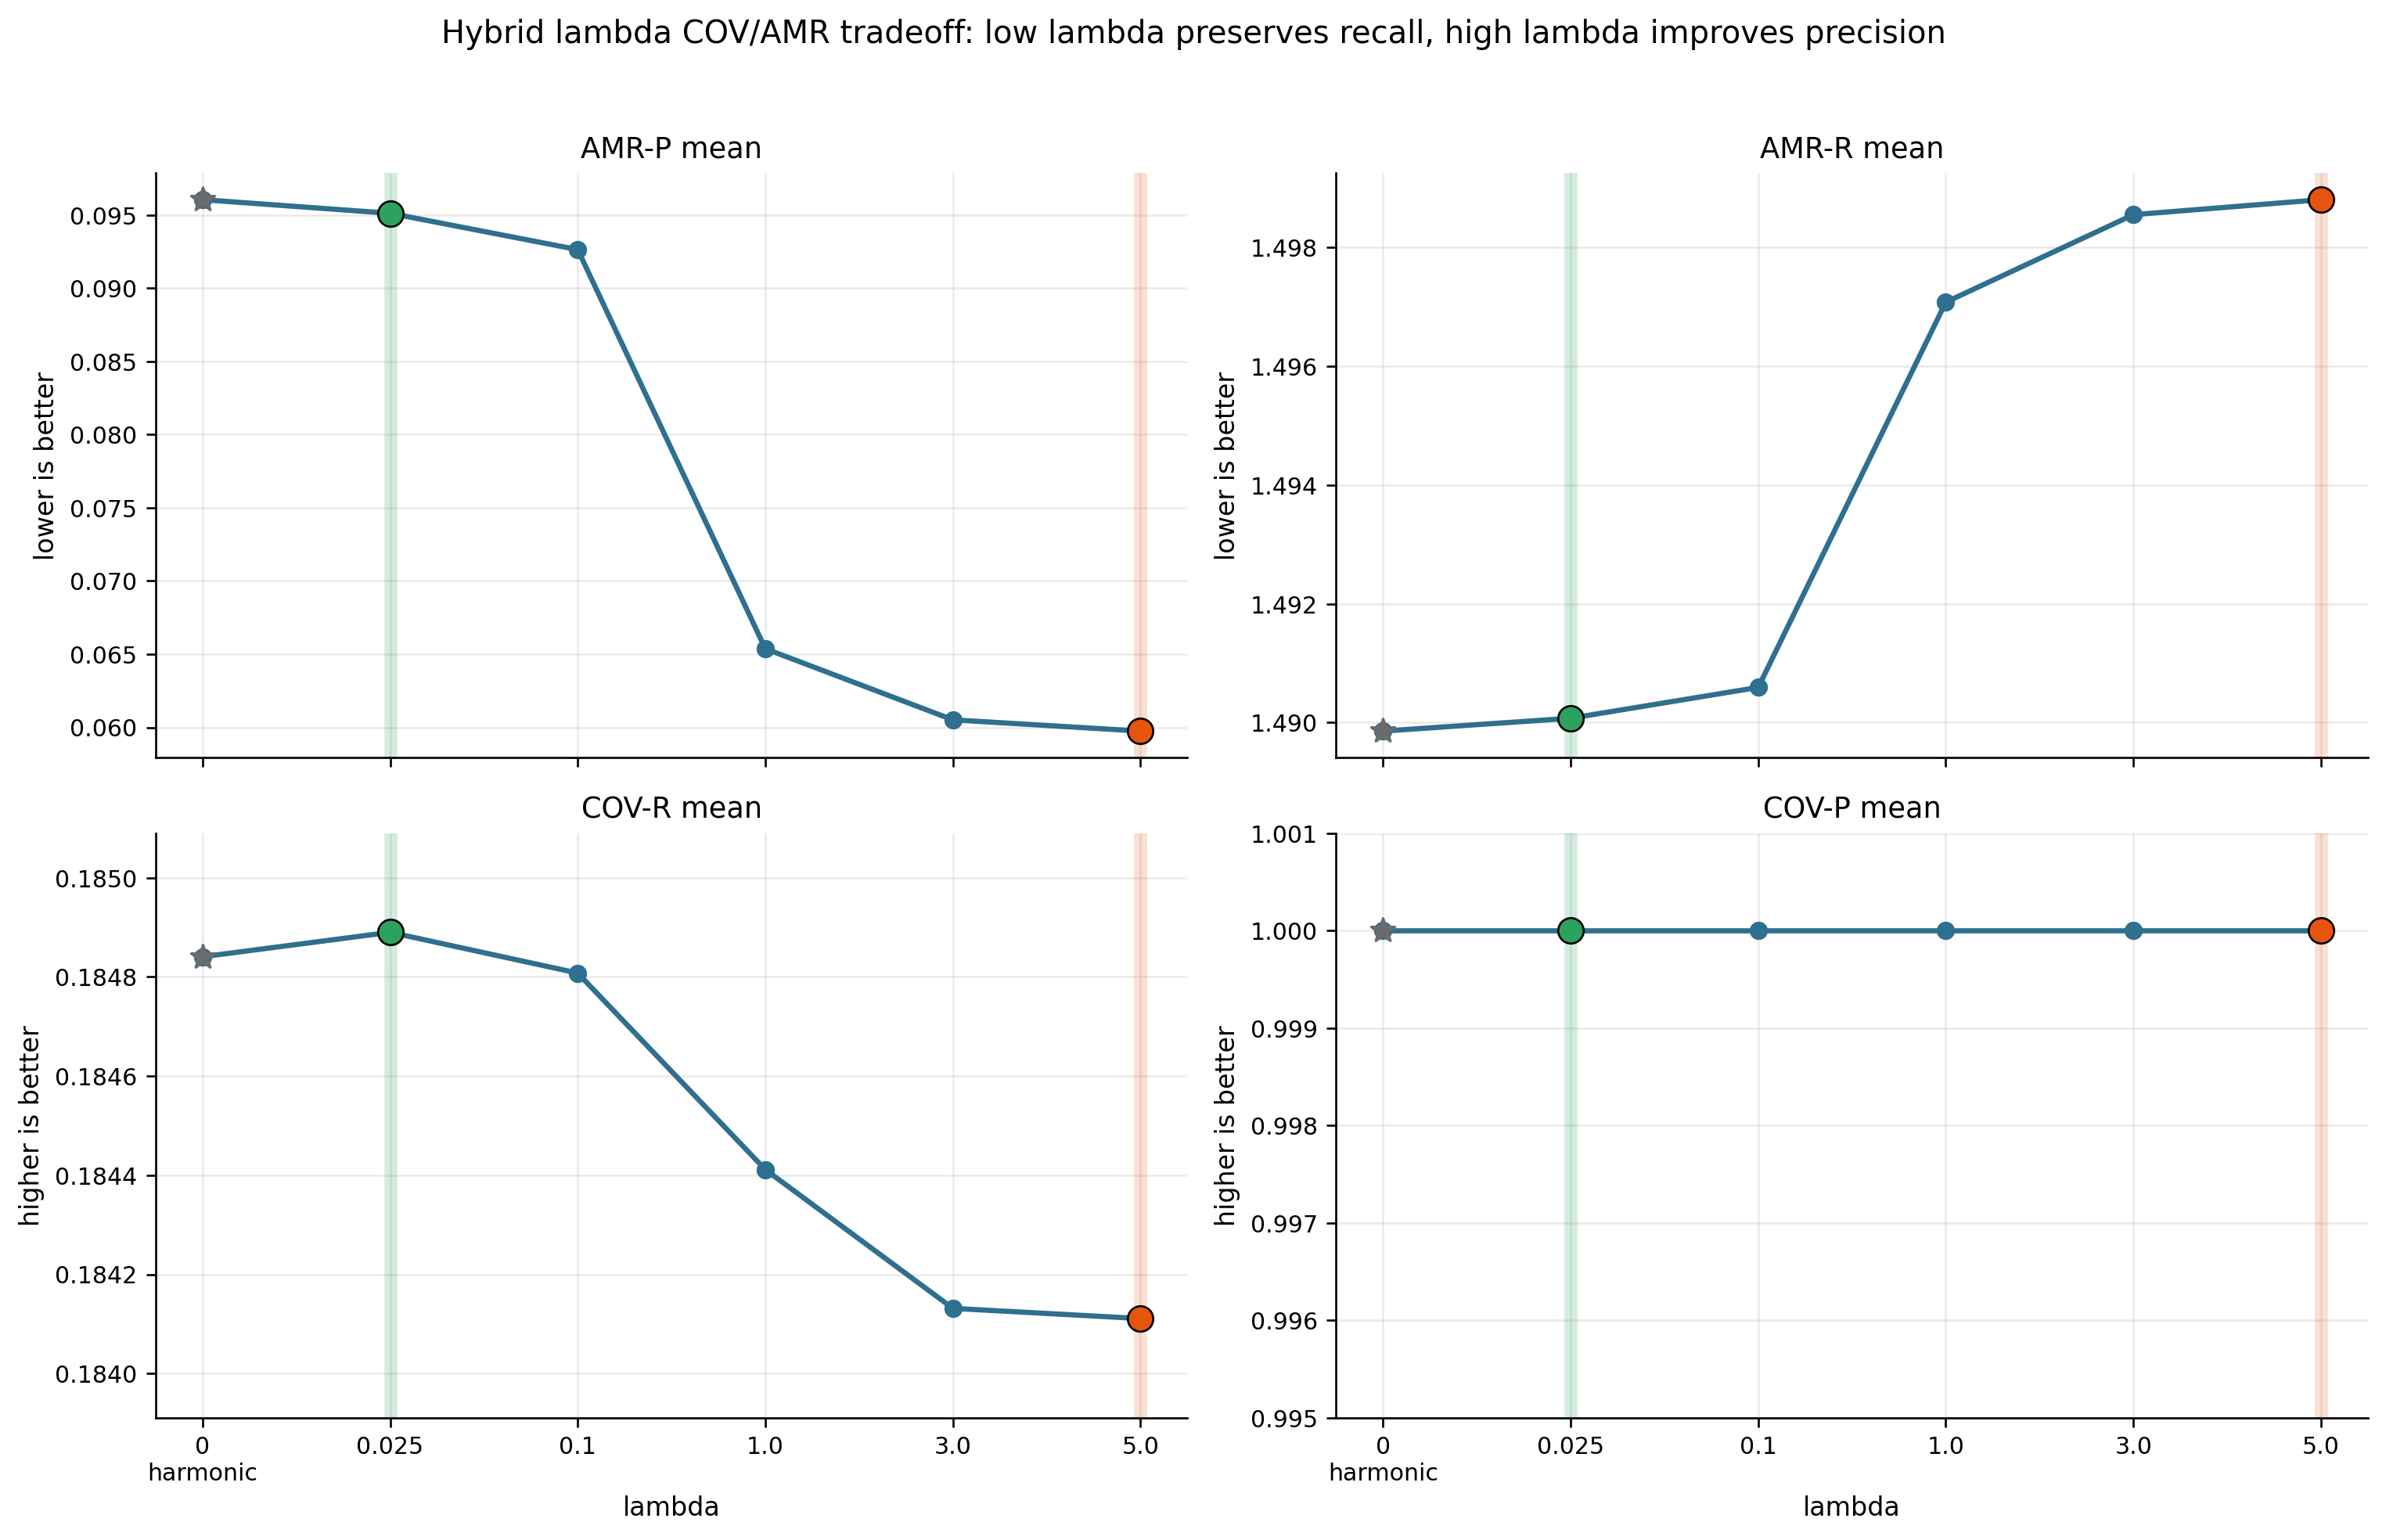
\includegraphics[width=0.95\linewidth]{geom_full_database_hybrid_lambda_cov_amr_tradeoff.png}
    \caption{Hybrid lambda tradeoff curve. Larger $\lambda$ improves AMR-P precision, while smaller $\lambda$ better preserves recall-style COV-R and AMR-R.}
    \label{fig:lambda-tradeoff}
\end{figure}

\begin{figure}[t]
    \centering
    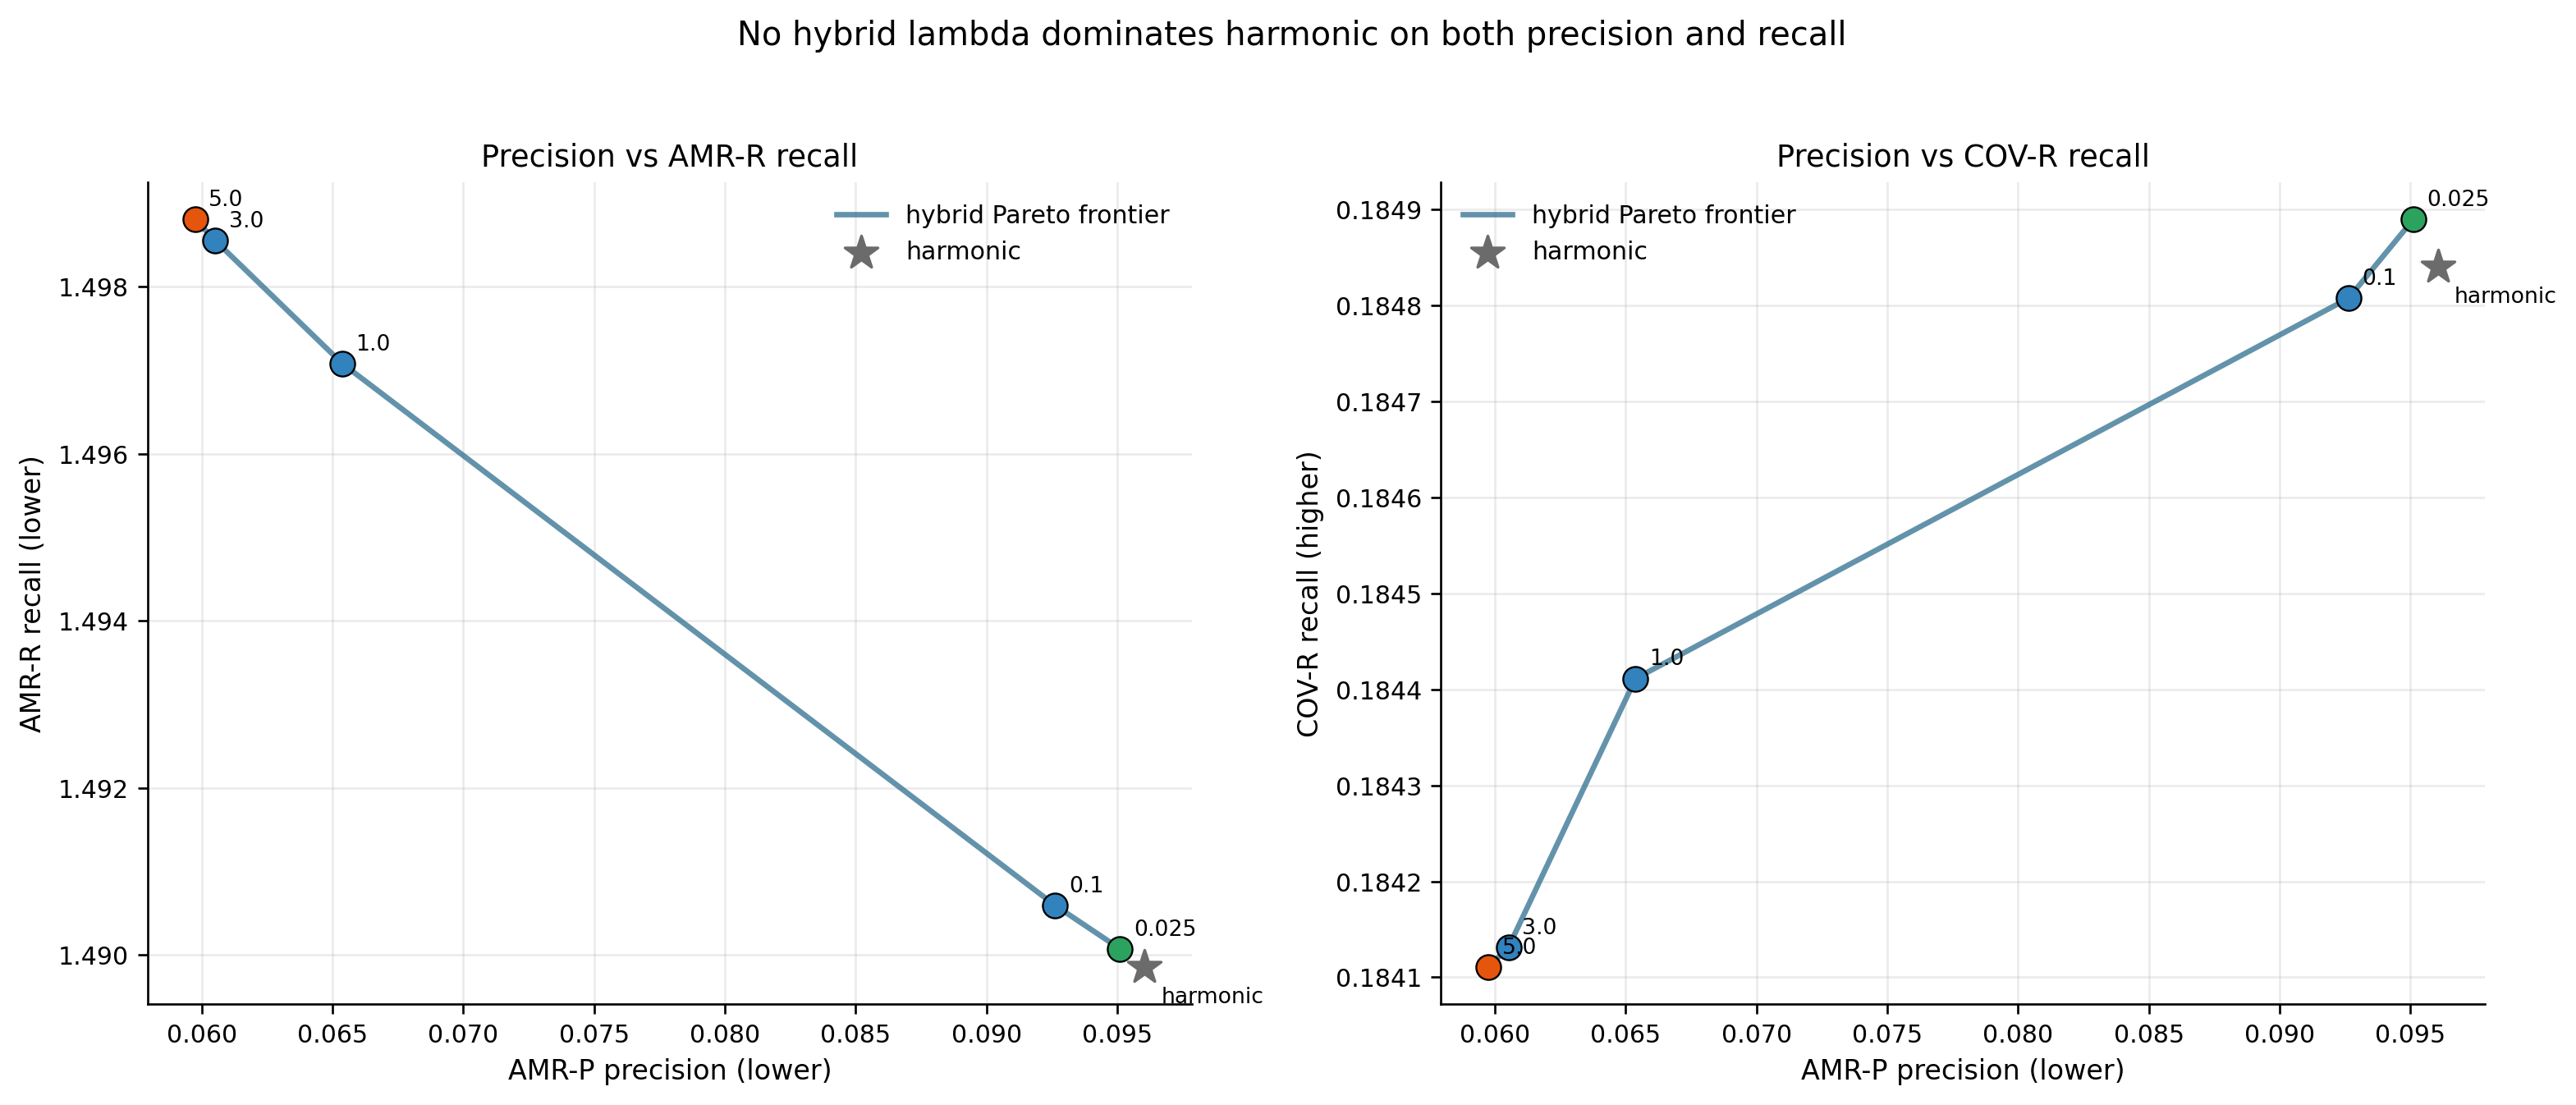
\includegraphics[width=0.85\linewidth]{geom_full_database_hybrid_lambda_precision_recall_pareto.png}
    \caption{Precision-recall Pareto plot from the final closure bundle. The final interpretation is a frontier rather than one universally best lambda.}
    \label{fig:pareto}
\end{figure}

\begin{figure}[t]
    \centering
    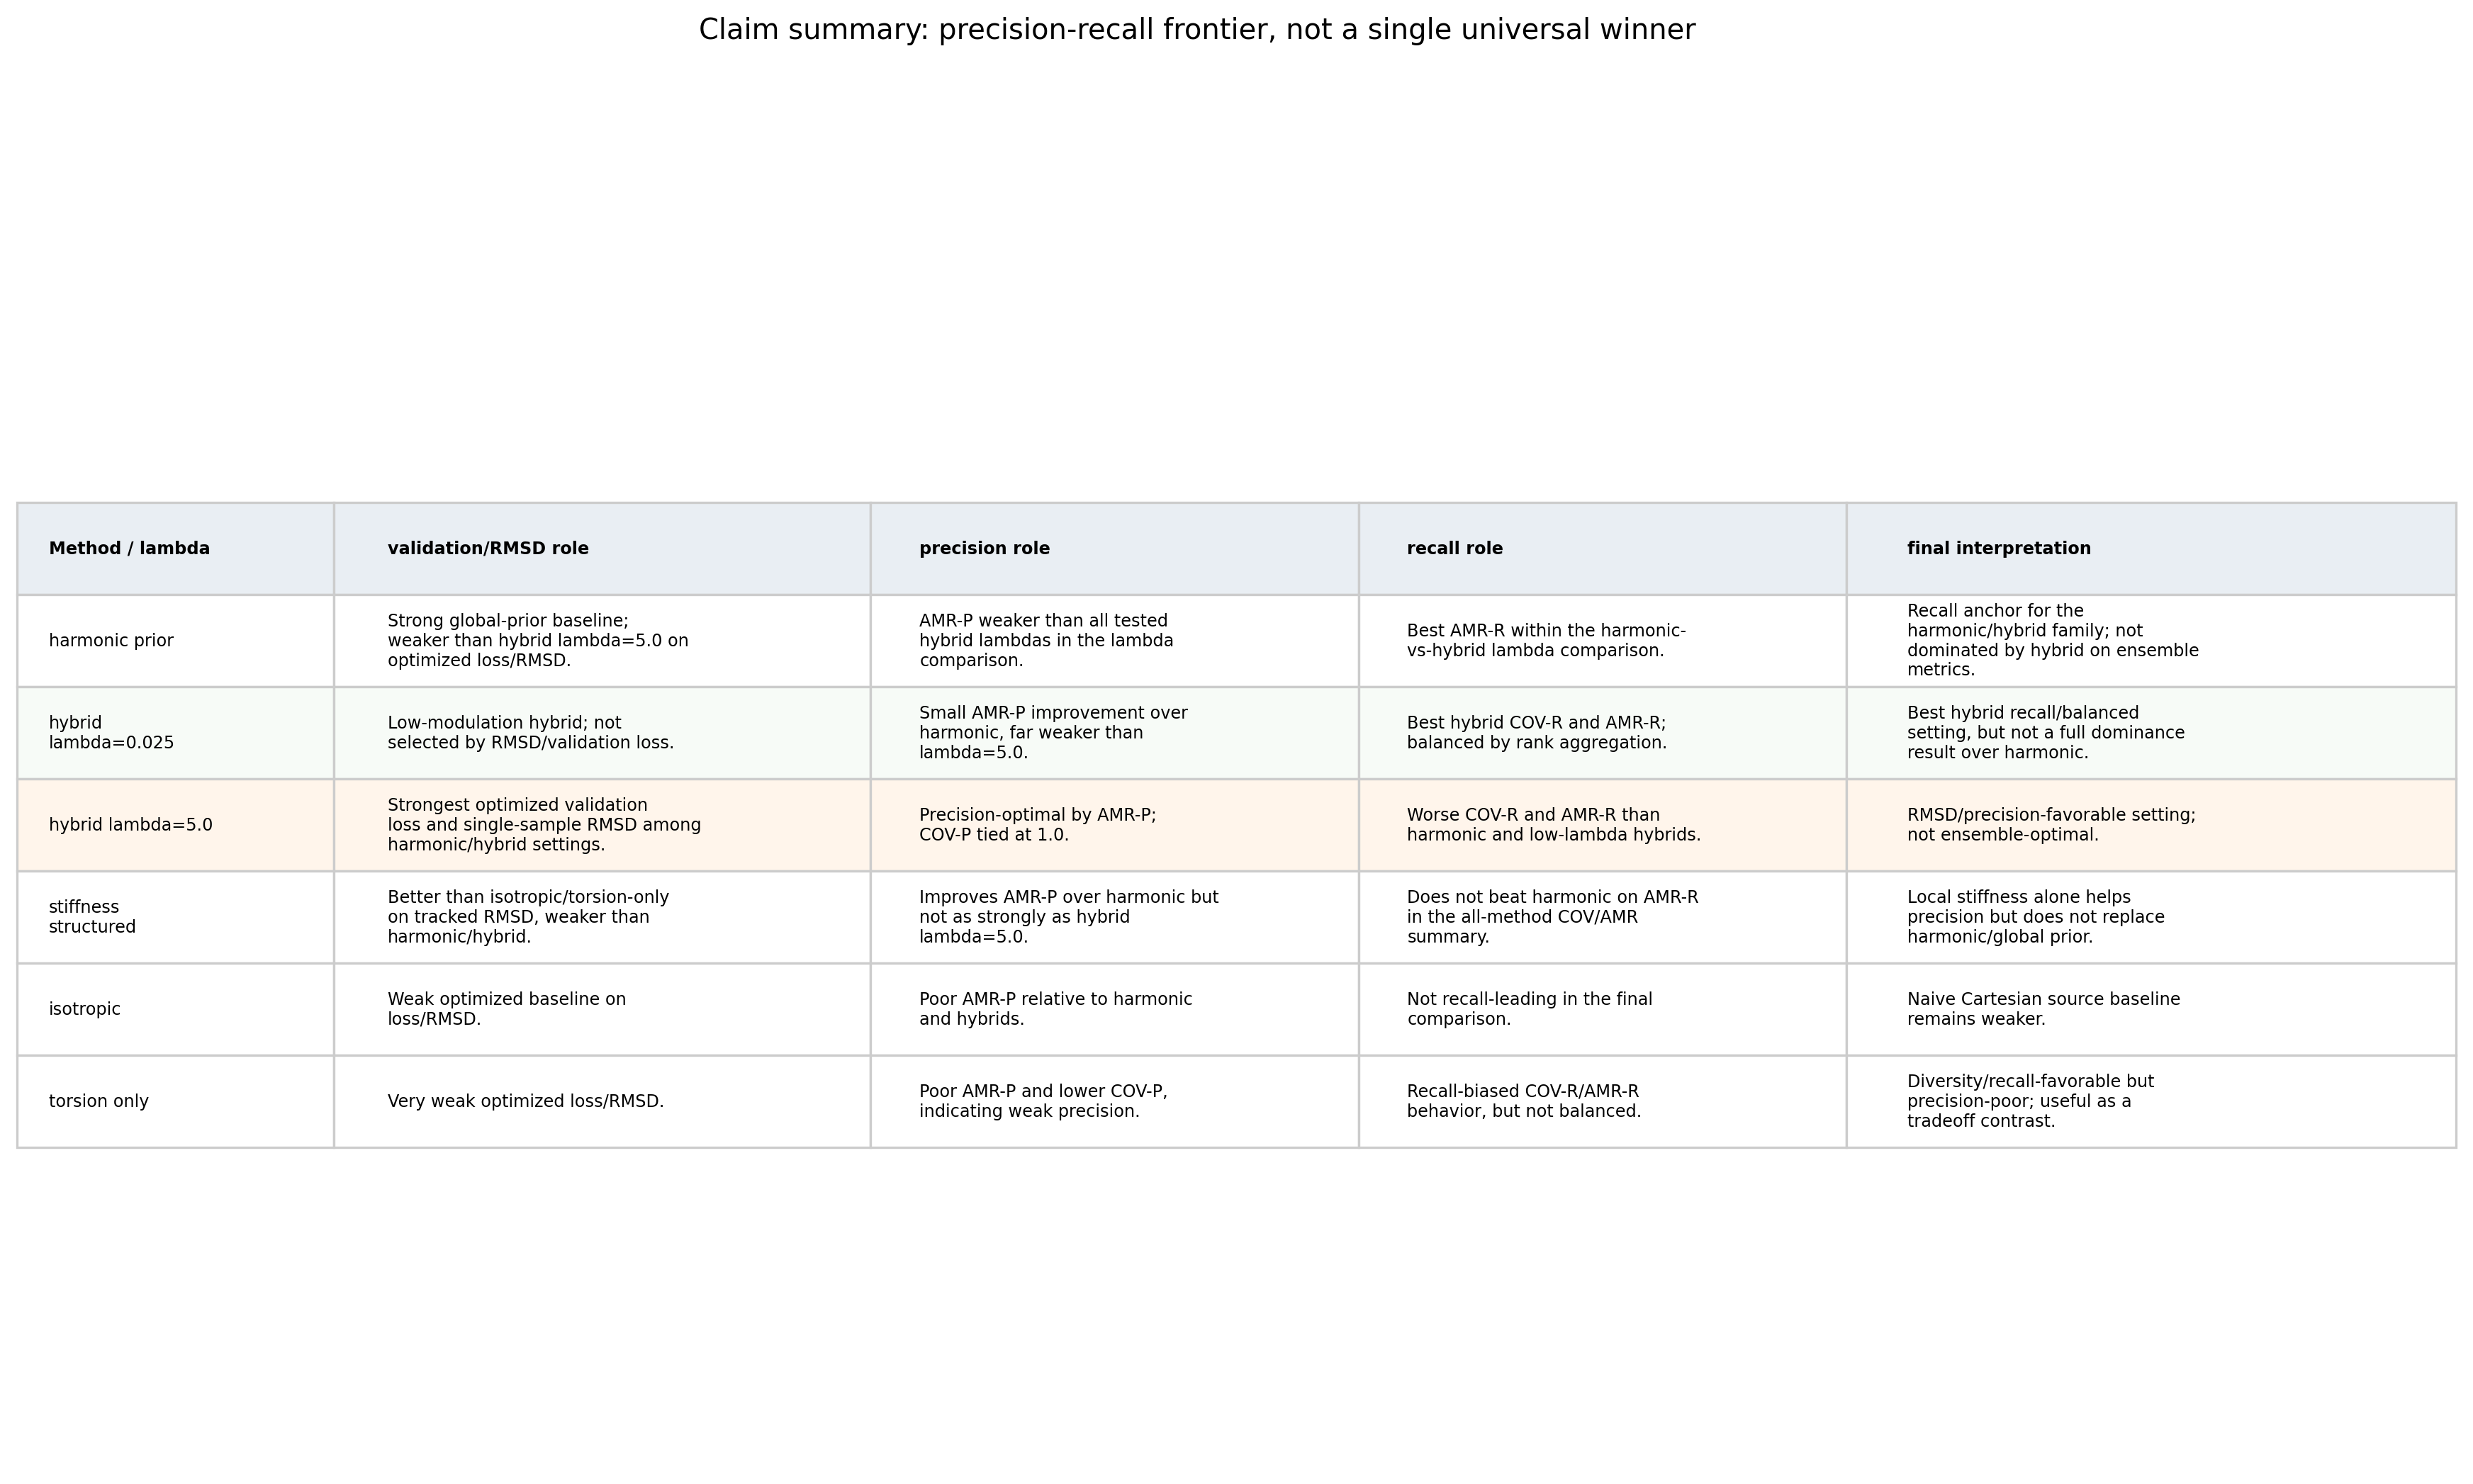
\includegraphics[width=0.95\linewidth]{geom_full_database_final_claim_summary_table.png}
    \caption{Claim summary table from the final reporting bundle. The table distinguishes validation/RMSD role, precision role, recall role, and final interpretation.}
    \label{fig:claim-table}
\end{figure}

\section{Discussion}

\subsection{Why Harmonic Is Strong}

The harmonic prior is strong because it contributes global geometric structure. Compared with isotropic noise, it likely gives a source distribution that is closer to the molecular conformer manifold and produces a shorter, easier transport problem. Compared with local stiffness rules alone, it captures broad geometric organization rather than only local rigidity or flexibility. This explains why stiffness-structured corruption alone improves over weaker baselines but remains worse than harmonic on tracked validation/RMSD metrics.

The result is consistent with the motivation from ET-Flow-style Cartesian approaches \cite{etflow}: one can stay in Cartesian coordinates while using a structured source prior. The project does not show that local stiffness replaces this global prior. It shows that local stiffness can modulate it in useful ways.

\subsection{What Stiffness Contributes}

Stiffness contributes local chemical structure. The rules protect rings, amide-like motifs, aromatic or conjugated regions when detectable, and bond/angle-sensitive neighborhoods, while allowing more variation around flexible groups. On its own, this improves over isotropic and torsion-only sources on tracked loss/RMSD metrics. When combined with the harmonic prior, it substantially improves single-sample RMSD and AMR-P precision.

This suggests that the harmonic prior and stiffness rules are complementary. The harmonic prior supplies the global source, while stiffness modulation changes where local variance is concentrated. The most useful high-lambda behavior is not simply lower noise everywhere. It appears to be a redistribution of source variability toward chemically softer regions and away from locally stiff regions.

\subsection{Precision-Recall Interpretation}

The final COV/AMR results support a precision-recall interpretation. High $\lambda$ makes generated conformers more precise with respect to nearby reference structures, which lowers AMR-P. At the same time, it reduces the ability to cover the reference ensemble as measured by COV-R and AMR-R. This is not necessarily a failure. A user may prefer high precision if downstream evaluation rewards a small number of accurate conformers. A different user may prefer recall if the goal is broad conformer coverage.

The important point is that metric choice changes lambda choice. If the target is validation loss or single-sample RMSD, $\lambda=5.0$ is the current best setting. If the target is balanced COV/AMR within the tested hybrid family, $\lambda=0.025$ is better. If the target is AMR-R recall in the harmonic-vs-hybrid family, harmonic remains the anchor.

\subsection{The Final Contribution Is a Source-Prior Family}

The clean contribution is a tunable family of source priors. This is more defensible than claiming a single best method. The results show that local stiffness information can improve a harmonic prior, but the improvement depends on which part of the conformer-generation problem is being measured.

This framing also protects the attribution. The same architecture and flow objective are used across the comparisons, and the intervention is source-only. The final method does not require a new architecture, a residual repair head, or a full internal-coordinate path. It instead exposes a controlled source-design knob that trades precision against recall.

\subsection{Limitations}

Several limitations remain.

First, this report does not claim full physical benchmark superiority. PoseBusters-style validity, MMFF/UFF energy or force sweeps, and xTB/GFN2-xTB checks were not completed as final evidence. Existing physical-validity notes in the repository are planning or proxy diagnostics, not a complete physical benchmark result.

Second, complete COV/AMR was computed on val/test partitions only. The train partition was excluded by design because it would make the evaluation much larger. This is appropriate for the final evaluation question, but it means the report should not be read as a train+val+test exhaustive ensemble analysis.

Third, the conclusions depend on the fixed architecture, objective, cached data processing, and final AdamW lr $10^{-3}$ protocol used here. A different backbone, flow path, or optimizer schedule could change the absolute values.

Fourth, lambda selection depends on the metric. The high-lambda hybrid is best for validation/RMSD and AMR-P precision, while the low-lambda hybrid is better for recall/balanced COV/AMR among tested hybrid settings. No tested hybrid lambda dominates harmonic on both precision and recall.

\section{Conclusion}

This project tested whether local stiffness rules can improve source construction for fixed-topology molecular conformer flow matching. The results support a careful conclusion. Local stiffness structure alone improves over isotropic and torsion-only sources on tracked validation/RMSD metrics, but harmonic remains stronger than stiffness alone. Combining stiffness modulation with the harmonic prior gives a stronger tracked validation/RMSD result: under AdamW lr $10^{-3}$, hybrid $\lambda=5.0$ beats optimized harmonic across random and scaffold splits and seeds 0, 1, and 2.

The ensemble evaluation is more nuanced. Complete val/test COV/AMR shows that $\lambda=5.0$ is precision/RMSD-favorable, especially through AMR-P, but it is not ensemble-optimal. A smaller hybrid lambda, $\lambda=0.025$, is recall/balanced-favorable among tested hybrids, and harmonic remains the AMR-R recall anchor in the harmonic-vs-hybrid comparison. The final conclusion is therefore a precision-recall frontier, not universal dominance. Stiffness-modulated harmonic priors are useful because they make this tradeoff controllable.

\appendix

\section{Reproducibility Pointer}

The final closure bundle is located at:
\begin{quote}
\path{reports/presentation_bundle/final_closure/}
\end{quote}

The final closure audit is located at:
\begin{quote}
\path{experiments/results/geom_full_database_project_closure_audit.json}
\end{quote}

The final report uses the following non-superseded summaries:
\begin{itemize}
    \item \path{experiments/results/geom_full_database_final_optimized_all_methods_summary.json}
    \item \path{experiments/results/geom_full_database_final_optimized_harmonic_vs_hybrid_summary.json}
    \item \path{experiments/results/geom_full_database_final_cov_amr_complete_valtest_summary.json}
    \item \path{experiments/results/geom_full_database_hybrid_lambda_complete_cov_amr_summary.json}
    \item \path{experiments/results/geom_full_database_final_hybrid_lambda_cov_amr_interpretation_summary.json}
    \item \path{experiments/results/geom_full_database_final_claims_and_limitations_summary.json}
\end{itemize}

To verify final-state consistency without running training or evaluation chunks, use:
\begin{verbatim}
python - <<'PY'
import json
paths = [
  "experiments/results/geom_full_database_final_hybrid_lambda_cov_amr_interpretation_summary.json",
  "experiments/results/geom_full_database_final_claims_and_limitations_summary.json",
  "experiments/results/geom_full_database_hybrid_lambda_complete_cov_amr_summary.json",
  "experiments/results/geom_full_database_final_cov_amr_complete_valtest_summary.json",
  "experiments/results/geom_full_database_final_optimized_all_methods_summary.json",
  "experiments/results/geom_full_database_project_closure_audit.json",
]
for path in paths:
    data = json.load(open(path))
    print(path, data.get("benchmark_result"), data.get("raw_data_modified"))
PY
\end{verbatim}

No scheduler submission, training, raw-data mutation, or environment mutation is needed to reproduce the final reporting bundle.

\section{Additional Notes on COV/AMR}

The complete hybrid-lambda COV/AMR evaluation was bounded to val/test partitions and used $K=20$ generated conformers per molecule. The final merged summary reports:
\begin{itemize}
    \item 2160/2160 expected tasks complete for the hybrid-lambda evaluation;
    \item 1,095,624 evaluated method-seed-molecule records;
    \item zero missing JSONL chunks;
    \item zero failed records;
    \item zero skipped records.
\end{itemize}

These details support the completeness of the COV/AMR reporting, but they do not make the result a physical benchmark. Physical validity checks remain a separate future step.

\bibliographystyle{plain}
\bibliography{references}

\end{document}
